% main.tex, to be used with thesis.tex
% This contains the main work of your thesis.

%\bibliography{thesis}  % uses the references stored in Chapter1Radar.bib

\chapter{Taxonomic Classification of Persistence Storage Systems for Sensor
Networks}
\label{chap:taxonomies}

Different mechanisms are used for persisting data collected from sensor
networks, as described by the section regarding the state of the art in sensor
networks and different approaches for persistence. This section analyzes these
approaches and presents the different approaches through 
taxonomy\footnote{Taxonomy is the practice and science of classification, by
using taxonomic units known as taxa (singular taxon)}, which will be used
throughout this work to evaluate different existing database systems
implementations, taking into account different requirements and specifications
of different sensor networks.

\section{Nature of Sensor Data Taxonomy}

No matter the type of resource management used, the first taxonomy presented is
related to the purpose of the use of the collected sensor data. That is, when
and how the collected data is going to be used as described in section
\ref{sec:sn-data-purpose}. In addition to it, the mechanism for data storage
described in section \ref{sec:sn-infrastructure} can be related to each of
them. The related taxon is depicted by figure \ref{fig:taxonomy-data-purpose}.

\begin{figure}[h]
  \centering
  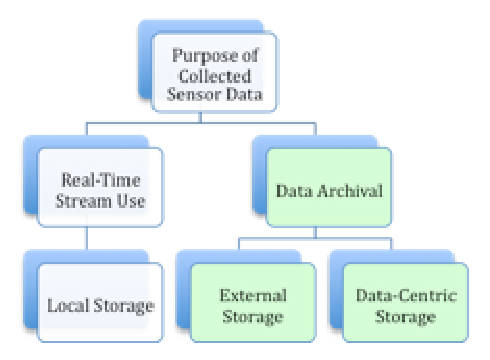
\includegraphics{../diagrams/taxonomy-data-purpose}
  \caption{The Nature and Location of Sensor Data Taxonomy}
  \label{fig:taxonomy-data-purpose}
\end{figure}

\begin{itemize}
  \item \textbf{Real-time Data Stream}: data is used as real-time data stream
  during data query \cite{sn-intro01};
  \item \textbf{Archival Data}: data is used for historical purposes such as
  data analysis or data fusion \cite{sn-intro01, sn-intro02}.
\end{itemize}

\section{Location of Sensor Data Taxonomy}

No matter the type of resource management used, the first taxonomy presented is
related to the purpose of the use of the collected sensor data. That is, when
and how the collected data is going to be used as described in section
\ref{sec:sn-data-purpose}. In addition to it, the mechanism for data storage
described in section \ref{sec:sn-infrastructure} can be related to each of
them. The related taxon is depicted by figure \ref{fig:taxonomy-data-location}.

\begin{figure}[h]
  \centering
  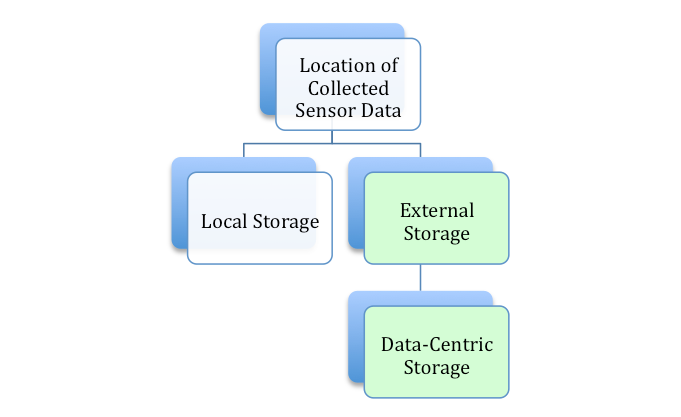
\includegraphics{../diagrams/taxonomy-data-location}
  \caption{The Nature and Location of Sensor Data Taxonomy}
  \label{fig:taxonomy-data-location}
\end{figure}

\begin{itemize}
  \item \textbf{Local Storage}: The data can be temporarily persisted
   in-memory, or a secondary memory device in a local storage device. It is
  directly related to the real-time data stream taxon, since it occurs at
  the place of the sensor device;
  \item \textbf{External Storage}: The data is usually located in an
  external storage device with a data management system such as a database
  system.
  \item \textbf{Data-Centric Storage}: the collected data can arranged in a
  categorized fashion as described by \cite{sn-storage03}. This taxon of
  system allows the data to be partitioned by a specific property. Nowadays,
  the strategy is often related to database partition \cite{db-partition}
  and database sharding approaches \cite{db-shard01} \cite{db-shard02}.
\end{itemize}

\section{Data Model Taxonomy}

One of the major challenges in the development of a persistence storage for
sensor network is related to the persistence model chosen. The addition of new
sensor devices may trigger refactoring of the existing model or not, depending
on how the data model accommodates the data. Different data models are reported
to be used in the literature, as described in section \ref{sec:data-models}.
For this reason, taxonomy related to the data model depicts two different
classes of data models, as shown in figure \ref{fig:taxonomy-data-model}.

\begin{figure}[h]
  \centering
  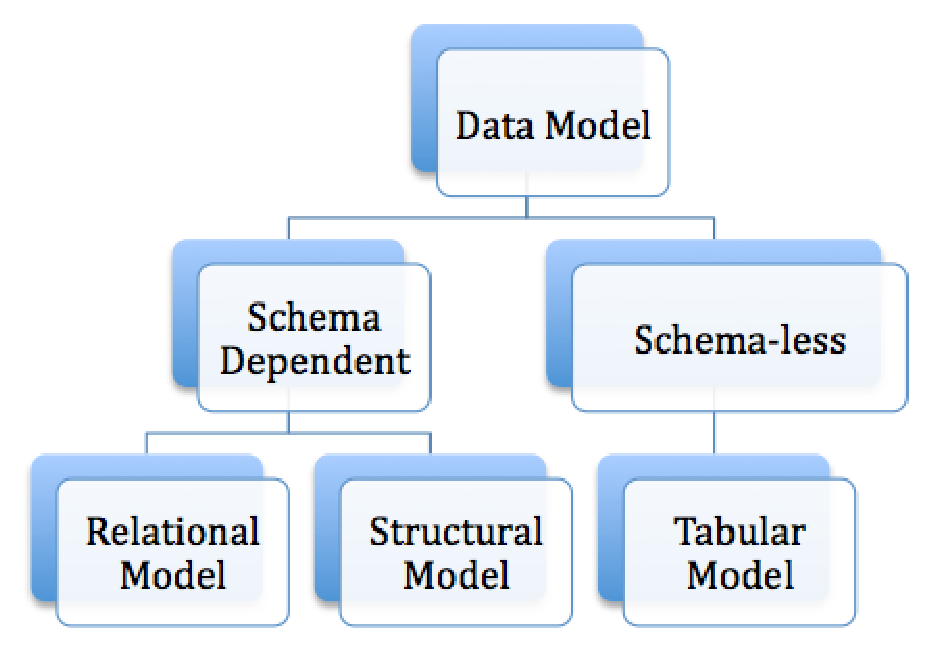
\includegraphics{../diagrams/taxonomy-data-model}
  \caption{Data Model Taxonomy}
  \label{fig:taxonomy-data-model}
\end{figure}

\begin{itemize}
  \item \textbf{Schema-Dependent Models}: this type of data model require
  the definition of a master schema that describes the data through a regorous
  data modeling process prior to the use of the data. In addition, an addition
 to a new sensor device, and consequently a new data entity, requires a
 re-evaluation of the existing data schema. For instance, relational model is
 governed by the relational algebra model, while the structured models such as
 XML needs a definition of an XML Schema.
  \item \textbf{Schema-less Models}: contrary to the previous taxon, 
  schema-less data models does not require the definition of a schema or master
  table definition and relationships. Instances of such data model is the KVP
  and the document-oriented models, whose usage in wireless sensor networks
  have not been reported.
\end{itemize}

\section{Data Provenance Taxonomy}

No matter the type of data model used, the support for Data Provenance as shown
in section \ref{sec:sn-provenance} is as important as the data being collected.
For this reason, the data model taxonomy must have support for the data types
that support the use of provenance-related attributes in the collected sensor
data. In this way, Figure \ref{fig:taxonomy-data-provenance} describes the data types
for the metadata support.

\begin{figure}[h]
  \centering
  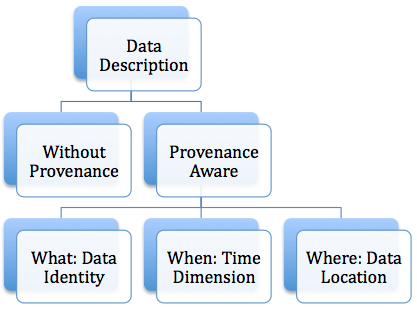
\includegraphics{../diagrams/taxonomy-data-provenance}
  \caption{Data Provenance Taxonomy}
  \label{fig:taxonomy-data-provenance}
\end{figure}

\begin{itemize}
  \item \textbf{What: Data Identity}: the data type that uniquely identifies
  the collected sensor dat;
  \item \textbf{When: Time Dimension}: the data type that identifies the
  collected data;
  \item \textbf{Where: Data Location}: an optional data type that identifies
  where the data came from.
\end{itemize}

\section{Query Processing Mechanism Taxonomy}

The query processing mechanism in sensor networks is directly related to how
and where the collected data is used and stored, as shown in the previous
section. As a consequence, the following taxonomy taxon is related to the
different types of query processing mechanisms described in section
\ref{sec:query-process}, and can be seen in figure
\ref{fig:taxonomy-query-mechanism}.

\begin{figure}[h]
  \centering
  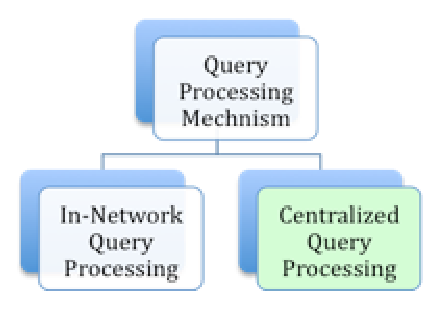
\includegraphics{../diagrams/taxonomy-query-mechanism}
  \caption{Query Processing Mechanism Taxonomy}
  \label{fig:taxonomy-query-mechanism}
\end{figure}

\begin{itemize}
  \item \textbf{In-Network Query Processing}: the sensor node receives a
  request to the properties of the sensor, and returns the current values
  related to them \cite{sn-intro01}.
  \item \textbf{Centralized Query Processing}: as it is done in regular single
  server relational databases, the data is collected to a centralized data
  sink in order to be used.
\end{itemize}

\section{Database System Organization Taxonomy}

Different approaches of data storage can also be related to the performance in
the database system used, and how its architecture provides the data storage
solution. For example, one important problem related to the centralized
network sink in sensor networks is the presence of an unavoidable creation of a
point of traffic concentration at the data collector or network nodes as
described by \cite{sn-storage02}. In this way, in order to mitigate the
problems associated with the so-called ``Funneling Effect", figure
\ref{fig:taxonomy-database-architecture} summarizes the different capabilities
of different types of database systems.

\begin{figure}[h]
  \centering
  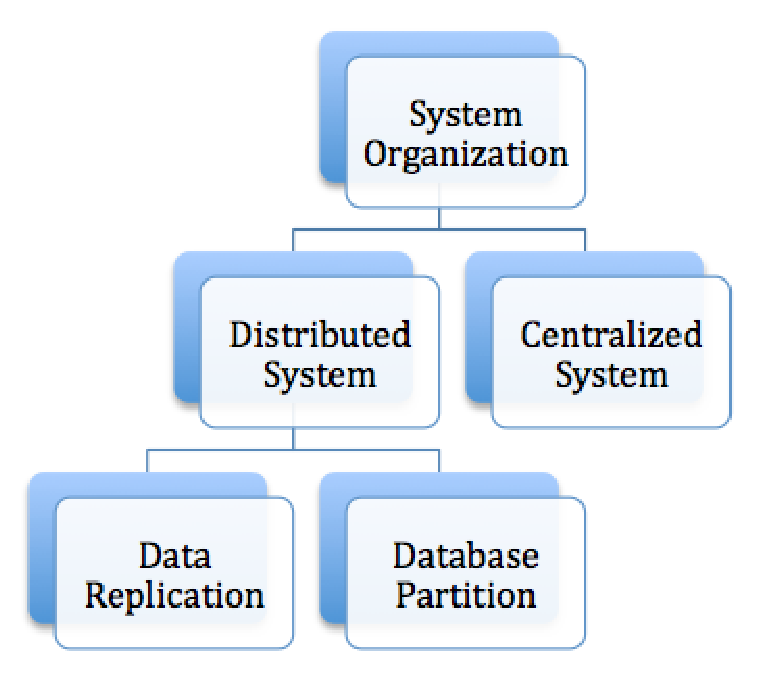
\includegraphics{../diagrams/taxonomy-database-architecture}
  \caption{Database Architecture Taxonomy}
  \label{fig:taxonomy-database-architecture}
\end{figure}

\begin{itemize}
  \item \textbf{Centralized System}: this is a database system that runs in
  one single centralized host, being the main point of data traffic as read
  and writes \cite{sn-intro01}.
  \item \textbf{Distributed System}: a database system that can be composed by
  more than one node. Usually, the use of the paradigm of Master-Slave
  mechanisms can be used by implementing ``Replication". In addition to it,
  ``Database Sharding" is used to portion the data related to a given shard
  key.
\end{itemize}